\documentclass{beamer}
\usepackage[utf8]{inputenc}
\usepackage{graphicx}
\usepackage{booktabs}
\usepackage{caption}
\usetheme{Madrid}
\usepackage{graphicx}
\usepackage{hyperref}
\usepackage{listings}
\usepackage{xcolor}

\title{PairCoder: A Multi-Agent Framework for Code Generation}
\author{Taylan Bapur, Jan H\"artrich}
\date{Summer 2025 -- Seminar on Machine Learning in Software Engineering}

\definecolor{codegray}{rgb}{0.5,0.5,0.5}
\lstdefinestyle{mystyle}{
    backgroundcolor=\color{white},
    commentstyle=\color{gray},
    keywordstyle=\color{blue},
    numberstyle=\tiny\color{codegray},
    stringstyle=\color{red},
    basicstyle=\ttfamily\footnotesize,
    breakatwhitespace=false,
    breaklines=true,
    captionpos=b,
    keepspaces=true,
    numbers=left,
    numbersep=5pt,
    showspaces=false,
    showstringspaces=false,
    showtabs=false,
    tabsize=2
}
\lstset{style=mystyle}





\begin{document}

\frame{\titlepage}

\begin{frame}{Overview}
\begin{itemize}
    \item Code generation with Large Language Models (LLMs) is improving, but challenges remain for complex tasks.
    \item \textbf{PairCoder} is a novel multi-agent system inspired by human pair programming.
    \item Compares favorably to Guided Code Generation and MapCoder.
\end{itemize}
\end{frame}

\begin{frame}{Motivation}
\begin{itemize}
    \item Single-agent LLMs struggle with:
    \begin{itemize}
        \item Complex reasoning
        \item Iterative debugging
        \item Backtracking and adaptation
    \end{itemize}
    \item Multi-agent systems aim to mitigate these issues by delegating roles.
\end{itemize}
\end{frame}

\begin{frame}{PairCoder Framework Overview}
\begin{itemize}
    \item Two agents: \textbf{Navigator} (planning) and \textbf{Driver} (execution).
    \item Iterative feedback loop until code passes test cases or max iterations.
\end{itemize}
\begin{center}
    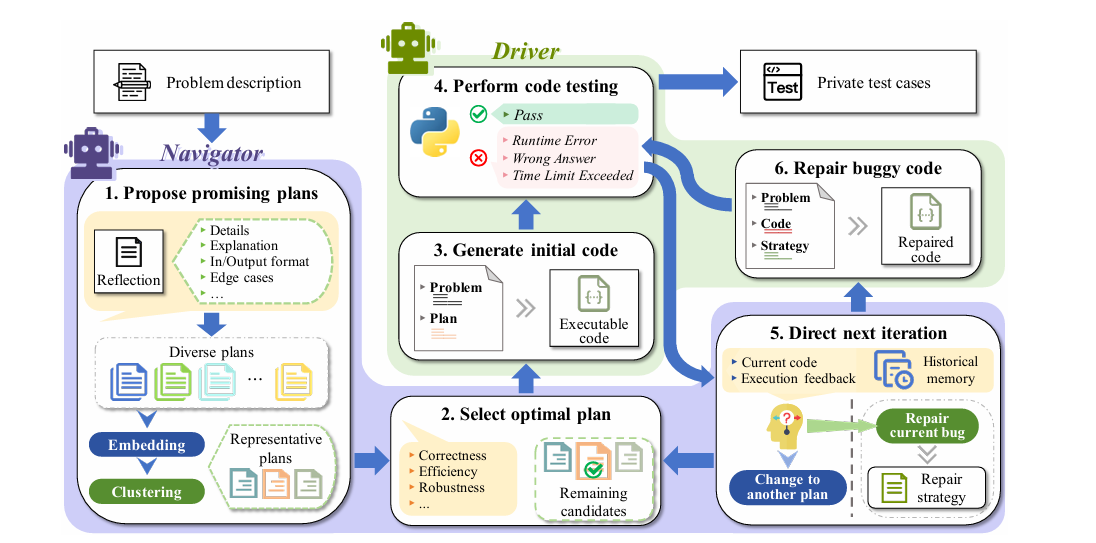
\includegraphics[width=0.95\textwidth]{paircoder-architecture.png}
\end{center}
\end{frame}

\begin{frame}{Navigator Agent}
\begin{itemize}
    \item Reflects on problem, input/output format, edge cases.
    \item Proposes multiple diverse solution plans.
    \item Uses semantic embeddings and k-means++ clustering.
    \item Tracks history to avoid redundant strategies.
\end{itemize}
\end{frame}

\begin{frame}{Driver Agent}
\begin{itemize}
    \item Stateless and reactive to Navigator's instructions.
    \item Implements selected plan into executable code.
    \item Tests code on public test cases.
    \item Applies repair strategies if needed.
\end{itemize}
\end{frame}

\begin{frame}{Core Techniques}
\textbf{Multi-Plan Exploration}
\begin{itemize}
    \item Diverse plans: brute force, greedy, DP, etc.
    \item Clustering avoids redundancy.
    \item Evaluation by correctness, efficiency, robustness.
\end{itemize}
\textbf{Feedback-Driven Refinement}
\begin{itemize}
    \item Results: Pass, Wrong Answer, Runtime Error, Time Limit Exceeded.
    \item Navigator chooses to repair or switch plans.
    \item Leverages historical memory.
\end{itemize}
\end{frame}

\begin{frame}{Evaluation Benchmarks}
\begin{itemize}
    \item \textbf{Benchmarks:} HumanEval, MBPP, CodeContest
    \item \textbf{Models:} GPT-3.5-Turbo, DeepSeek-Coder
    \item Measured using \texttt{pass@1} (pass all private tests on first try).
\end{itemize}
\end{frame}

\begin{frame}{Performance Results}
\begin{center}
    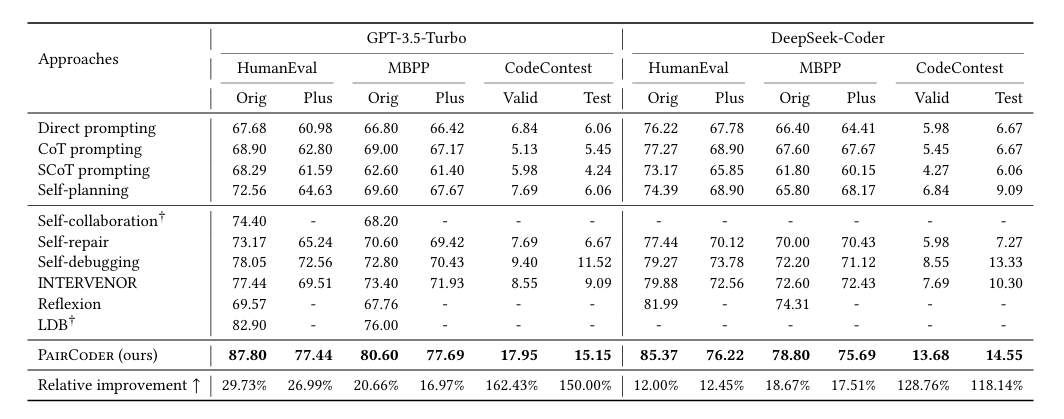
\includegraphics[width=0.95\textwidth]{paircoder-results.png}
\end{center}
\begin{itemize}
    \item PairCoder outperforms all baselines.
    \item Up to \textbf{87.80\%} pass@1 on HumanEval with GPT-3.5.
    \item Up to \textbf{162.43\%} improvement over prompting baselines.
\end{itemize}
\end{frame}

\begin{frame}{Ablation Studies}
\begin{itemize}
    \item \textbf{Without multi-plan:} 6--8\% accuracy drop.
    \item \textbf{Without feedback refinement:} 10--12\% drop.
    \item Confirms both components are crucial.
\end{itemize}
\end{frame}

\begin{frame}{Comparison: Guided Code Generation}
\begin{itemize}
    \item Hierarchical planning tree using Generalist, Code, and Tester agents.
    \item Modular and interpretable.
    \item Strong on compositional logic, but complex to manage.
    \item PairCoder is better for fast, flexible tasks.
\end{itemize}
\end{frame}

\begin{frame}{Comparison: MapCoder}
\begin{itemize}
    \item 4 agents: Retrieval, Planning, Coding, Debugging.
    \item Simulates full software development lifecycle.
    \item Adds plan scoring and algorithm tutorials.
    \item Strong modularity but dependent on high-quality examples.
\end{itemize}
\end{frame}

\begin{frame}{Threats to Validity}
\begin{itemize}
    \item Dataset leakage (e.g., HumanEval overlap)
    \item Prompt sensitivity and model size bias
    \item Benchmark limitations (single-function only)
    \item Pass@1 does not reflect partial correctness
    \item Reproducibility challenges noted in GitHub testing
\end{itemize}
\end{frame}


\begin{frame}[fragile]{Example: Bug Fixing and Plan Refinement}
\textbf{Original buggy implementation:}
\begin{verbatim}
def solve_buggy(arr):
    # Bug: Possible IndexError due to arr[i+1] access
    operations = 0
    for i in range(len(arr)):
        if arr[i] > i + 1 and arr[i+1] < arr[i]:
            operations += 1
    return operations
\end{verbatim}
\end{frame}

\begin{frame}[fragile]{Example: Bug Fixing and Plan Refinement}
\textbf{Refined (corrected) version:}
\begin{verbatim}
def solve_fixed(arr):
    arr = arr[:]
    i = 0
    ops = 0
    while i < len(arr):
        if arr[i] > i + 1:
            arr.insert(i, i + 1)
            ops += 1
        else:
            i += 1
    return ops
\end{verbatim}
\end{frame}



\begin{frame}{Discussion and Limitations}
\begin{itemize}
    \item PairCoder mimics human problem-solving effectively.
    \item Relies heavily on good initial plan diversity.
    \item Computationally more expensive than single-pass methods.
    \item Real-world usability depends on further optimization and robustness.
\end{itemize}
\end{frame}

\begin{frame}{Future Work}
\begin{itemize}
    \item Combine PairCoder's refinement with Guided Code’s hierarchy.
    \item Human-in-the-loop selection and interpretation.
    \item Cross-domain application (e.g., theorem proving).
    \item Dynamic test suite generation.
\end{itemize}
\end{frame}

\begin{frame}{Conclusion}
\begin{itemize}
    \item Multi-agent systems like PairCoder outperform single-agent LLMs.
    \item Iterative refinement and plan diversity are key strengths.
    \item Hybrid systems may offer even better performance.
    \item Continued work needed on implementation, reproducibility, and scalability.
\end{itemize}
\end{frame}

\end{document}